\documentclass[11pt]{beamer}
\usetheme{Boadilla}
%\usetheme{Berlin}
\usecolortheme{seahorse}
%\usecolortheme{beetle}
\usepackage[utf8]{inputenc}
\usepackage{amsmath}
\usepackage{amsfonts}
\usepackage{amssymb}
\usepackage{natbib}
\usepackage{tcolorbox}
\usepackage{multimedia}
\newcommand{\dif}{\mathrm{d}}
\usepackage{graphicx}
\graphicspath{{Images/}}
\usepackage{media9}
\addmediapath{Animations/}
\newcommand{\folds}{(x_0,y_0)}
\newcommand{\st}{such that }
\newcommand{\wrt}{with respect to }
\newcommand{\vdp}{Van der Pol }
\newcommand{\wlg}{without loss of generality }
\newcommand{\Wlg}{Without loss of generality }


\begin{document}
  

\author{Jonna, Tom, Kieran}
\title{Fast and Slow Dynamics}
%\setbeamercovered{transparent} 
%\setbeamertemplate{navigation symbols}{} 
%\logo{} 
\institute{MIGSAA} 
\date{16/11/2018} 
%\subject{} 
\frame \titlepage
\begin{frame}
\begin{itemize}
\item Dynamical Systems and \vdp
\item Canards in the \vdp 
\item Mixed Mode Oscillations (MMO) 
%\item Canard Points
\end{itemize}

\end{frame}


\begin{frame}{ A Quick Reminder: Dynamical Systems}
\begin{onlyenv}<1>
%	\scalebox{1.5}{
\huge
 \[\begin{cases}
 \frac{\dif x}{\dif t}= -y + x^2 - \frac{x^3}{3}\\
 \frac{\dif y}{\dif t}=\epsilon (-\lambda+x)
 \end{cases}\]%}
\end{onlyenv}
\begin{onlyenv}<2>
\begin{columns}
\column{0.6\textwidth}
\begin{figure}
    \centering
\includemedia[width=1\linewidth,height=1\linewidth,activate=pageopen,
passcontext,
transparent,
addresource=vdPe001.mp4,
flashvars={source=vdPe001.mp4}
]{}{VPlayer.swf}
\end{figure}
\column{0.4\textwidth}
\[\begin{cases}
 \frac{\dif x}{\dif t}= -y + x^2 - \frac{x^3}{3}\\
 \frac{\dif y}{\dif t}=\epsilon (-\lambda+x)
 \end{cases}\]
\end{columns}
\end{onlyenv}
\end{frame} 

\begin{frame}{The Van der Pol Equations}
\begin{columns} 
\column{0.5\textwidth}
\begin{figure}
    \centering
\includemedia[width=1\linewidth,height=1\linewidth,activate=pageopen,
passcontext,
transparent,
addresource=vdPe02.mp4,
flashvars={source=vdPe02.mp4}
]{}{VPlayer.swf}
    \caption{Phase Plane of the Van der Pol Equations}
\end{figure}


\column{0.5\textwidth}
\begin{itemize}
    %\item Van der Pol Equations, $\epsilon \rightarrow 0$
    \item Fast System:
    \begin{equation*} 
        % \begin{aligned} 
        \begin{cases}
        \frac{\dif x}{\dif t}&= -y + x^2 - \frac{x^3}{3}\\
        \frac{\dif y}{\dif t}&=\epsilon (-1+x)
        \end{cases}
        % \end{aligned}
        \end{equation*}
\pause
\item Slow System:\\
     \begin{itemize}\item Let $t=\frac{\tau}{\epsilon}$.\end{itemize}
\begin{equation*} 
        \begin{cases}
        \epsilon\frac{\dif x}{\dif \tau} &= -y + x^2 - \frac{x^3}{3}\\ 
        \frac{\dif y}{\dif \tau}&= (-1+x)
        \end{cases}
        \end{equation*}
\newline
\item Equilibrium 
\begin{itemize}
\item $(x_0,y_0)=(1,\frac{2}{3}) $
\end{itemize}
\end{itemize}
\end{columns}
\end{frame}


\begin{frame}{The Van der Pol Equations, $\epsilon=0$}
\begin{columns} 
\column{0.5\textwidth}
\begin{figure}
    \centering
\includemedia[width=1\linewidth,height=1\linewidth,activate=pageopen,
passcontext,
transparent,
addresource=vdPe001.mp4,
flashvars={source=vdPe001.mp4}
]{}{VPlayer.swf}
    \caption{Phase Plane of the Van der Pol Equations}
\end{figure}
\column{0.5\textwidth}
\begin{itemize}
  
    \item Layer Problem:
    \begin{equation*}
        \begin{cases}
        \frac{\dif x}{\dif t}&= -y + x^2 - \frac{x^3}{3}\\
        \frac{\dif y}{\dif t}&=0
        \end{cases}
        \end{equation*}

\item Reduced System:
\begin{equation*} 
        \begin{cases}
        0 &= -y + x^2 - \frac{x^3}{3}\\ 
        \frac{\dif y}{\dif\tau}&= (-1+x)
        \end{cases}
        \end{equation*}

\end{itemize}
\end{columns}
\end{frame}



\begin{frame}{The Reduced System}
\begin{columns}
\column{0.5\textwidth}
\begin{figure}
    \centering
\includemedia[width=1\linewidth,height=1\linewidth,activate=pageopen,
passcontext,
transparent,
addresource=vdPe001.mp4,
flashvars={source=vdPe001.mp4}
]{}{VPlayer.swf}
    \caption{Phase Plane of the Van der Pol Equations}
\end{figure}
\column{0.5\textwidth}
Reduced System:
\begin{equation*} 
        \begin{cases}
        0 &= -y + x^2 - \frac{x^3}{3} := f(x,y)\\ 
        \frac{\dif y}{\dif \tau}&= (-1+x)
        \end{cases}
        \end{equation*}
\newline
Nullcline:
\begin{align*}
 &y = x^2 - \frac{x^3}{3}
\end{align*}
\newline
\newline
Fold Points:
\begin{itemize}
\item$(x_1^*,y_1^*)= (0,0) $

\item$(x_2^*,y_2^*)=(2,\frac{4}{3})$
\end{itemize}


\end{columns}
\end{frame}


\begin{frame}{The Van der Pol Equations near $(x_1^*,y_1^*)$ }
\begin{columns}
\column{0.5\textwidth}
\begin{figure}[h!]
    \centering
    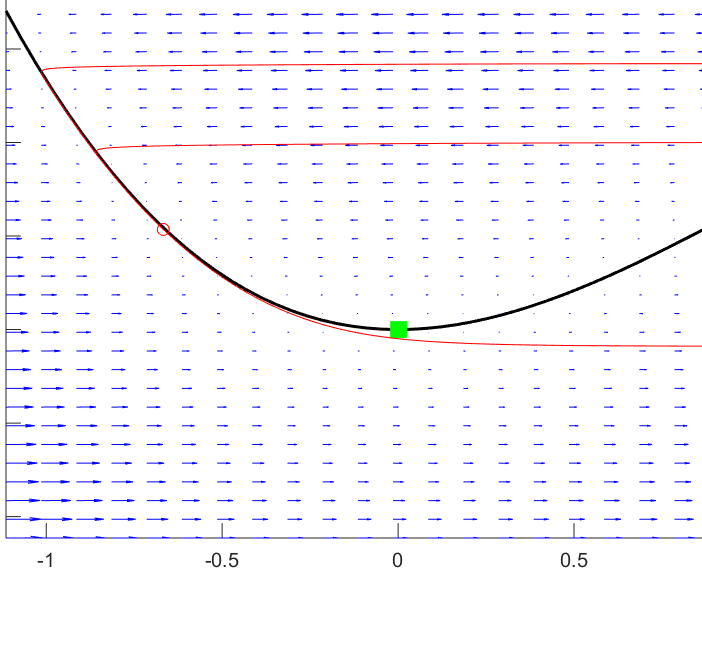
\includegraphics[width=\textwidth]{PPlanecrop.png}
\end{figure}
\column{0.5\textwidth}


Investigating Hyperbolicity:
\begin{align*}
f(x,y)&= -y + x^2 - \frac{x^3}{3}\\
\Rightarrow \frac{\dif f}{\dif x}&= 2x -x^2 \\
&= x(2-x)
\end{align*}
\newline
\newline
Fold Point $(x_1^*,y_1^*)= (0,0) $ is non-hyperbolic.
\end{columns}
\end{frame}

\begin{frame}{The Van der Pol Equations near $(x_1^*,y_1^*)$}
\begin{columns}
\column{0.5\textwidth}
\begin{figure}[h!]
    \centering
    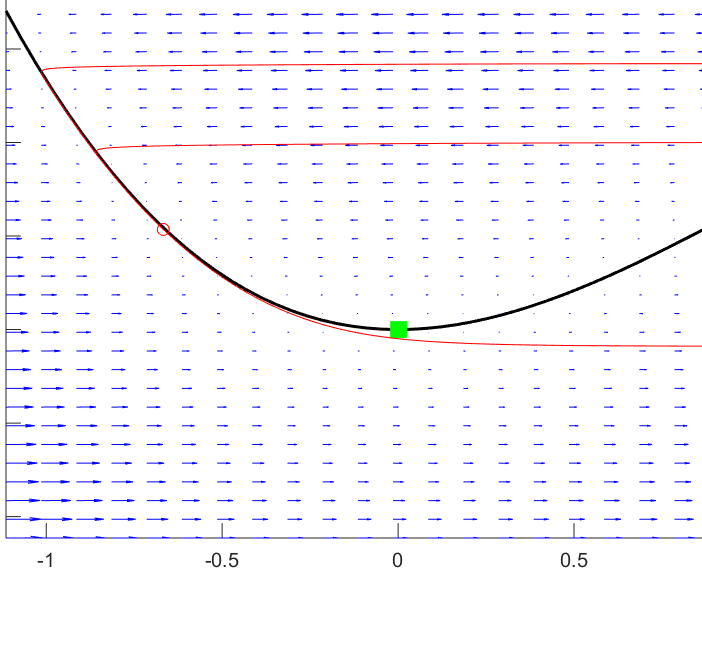
\includegraphics[width=\textwidth]{PPlanecrop.png}
\end{figure}
\column{0.5\textwidth}
Fold Point $(x_1^*,y_1^*)= (0,0) $  
\newline
is non-hyperbolic.
\begin{align*}
y&= x^2 - \frac{x^3}{3}\\
\Rightarrow \frac{\dif y}{\dif \tau}  &= \frac{\dif y}{\dif x} \frac{\dif x}{\dif\tau}  = x(2-x)\frac{\dif x}{\dif\tau}\\
\Rightarrow \frac{\dif x}{\dif\tau}&= \frac{\dif y}{\dif\tau}\frac{1}{(2-x)x}
\end{align*}
\newline
%\vspace{0.5cm}
Singularities at $x=0,x=2$.
\end{columns}
\end{frame}

\begin{frame}{Canard Points in the \vdp}
%\begin{onlyenv}<1>
%	\begin{equation*} 
%	\begin{cases}
%	\epsilon\frac{\dif x}{\dif \tau} &= -y + x^2 - \frac{x^3}{3}\\ 
%	\frac{\dif y}{\dif \tau}&= (-1+x)
%	\end{cases}
%	\end{equation*}
%\end{onlyenv}
%
%\begin{onlyenv}<2>
%	\begin{equation*}
%	\begin{cases}
%	\epsilon\frac{\dif x}{\dif \tau} &= -y + x^2 - \frac{x^3}{3}\\ 
%	\frac{\dif y}{\dif \tau}&= (-\lambda+x)
%	\end{cases}
%	\end{equation*}
%\end{onlyenv}
%
%\begin{onlyenv}<3>
	\begin{columns}
		\column{0.5\textwidth}
		\begin{figure}
			\centering
			\includemedia[width=1\linewidth,height=1\linewidth,activate=pageopen,
			passcontext,
			transparent,
			addresource=vdPhopf.mp4,
			flashvars={source=vdPhopf.mp4}
			]{}{VPlayer.swf}
			
		\end{figure}
		\column{0.5\textwidth}
		\begin{figure}
			\centering
			\includemedia[width=1\linewidth,height=1\linewidth,activate=pageopen,
			passcontext,
			transparent,
			addresource=vdPe001.mp4,
			flashvars={source=vdPe001.mp4}
			]{}{VPlayer.swf}
			%\caption{Phase Plane of the Van der Pol Equations}
		\end{figure}
	
	\end{columns}
	\begin{equation*} 
	\begin{cases}
	\epsilon\frac{\dif x}{\dif \tau} &= -y + x^2 - \frac{x^3}{3}\\ 
	\frac{\dif y}{\dif \tau}&= (-\lambda+x)
	\end{cases}
	\end{equation*}
\end{frame}

\begin{frame}{The Blow-up}
\begin{columns}
\column{0.5\textwidth}
\begin{figure}
    \centering
    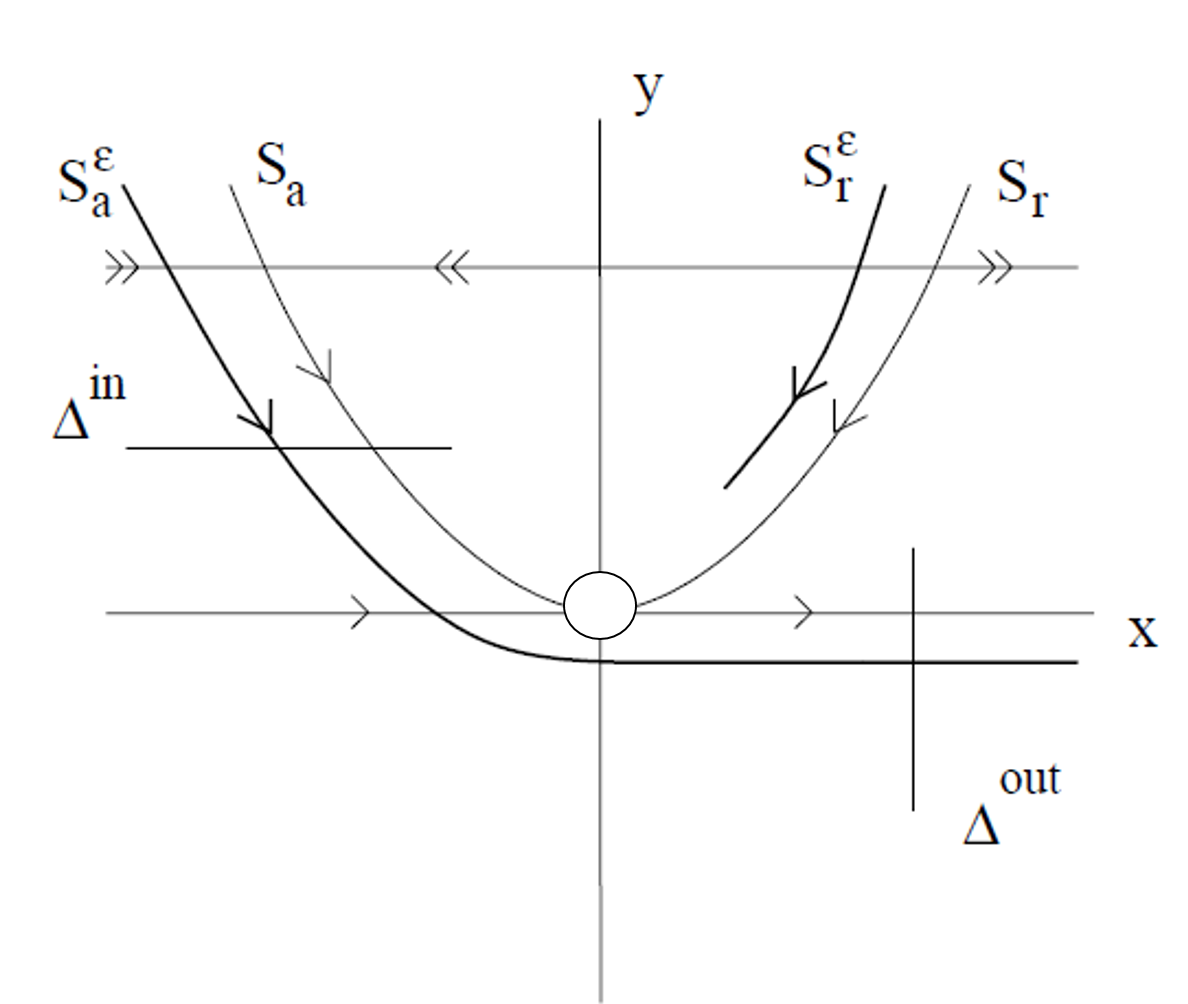
\includegraphics[height=5cm, width=5cm]{Blow_up.png}
    \caption{Blow up of our fold point (Kuehn, Multiple Time Scale Dynamics)}
\end{figure}\column{0.5\textwidth}

\begin{itemize}

\item The radius $r=0$
\item Coordinate transformation
\begin{itemize}
    \item $x=r_ix_i, \ y=r_i^2y_i, \ \epsilon=r_i^3\epsilon_i \ \lambda=r_i\lambda_i$\\
\end{itemize}
%\item Letting $r$ go to zero to describe flow on surface of blown up point $(x_1*,y_1*)$.
\item Analysing our blow up
\end{itemize}
\end{columns}
\end{frame}

\begin{frame}{Charts Motivation}
    \begin{columns}
     \column{0.5\textwidth}
    \begin{figure}
        \centering
        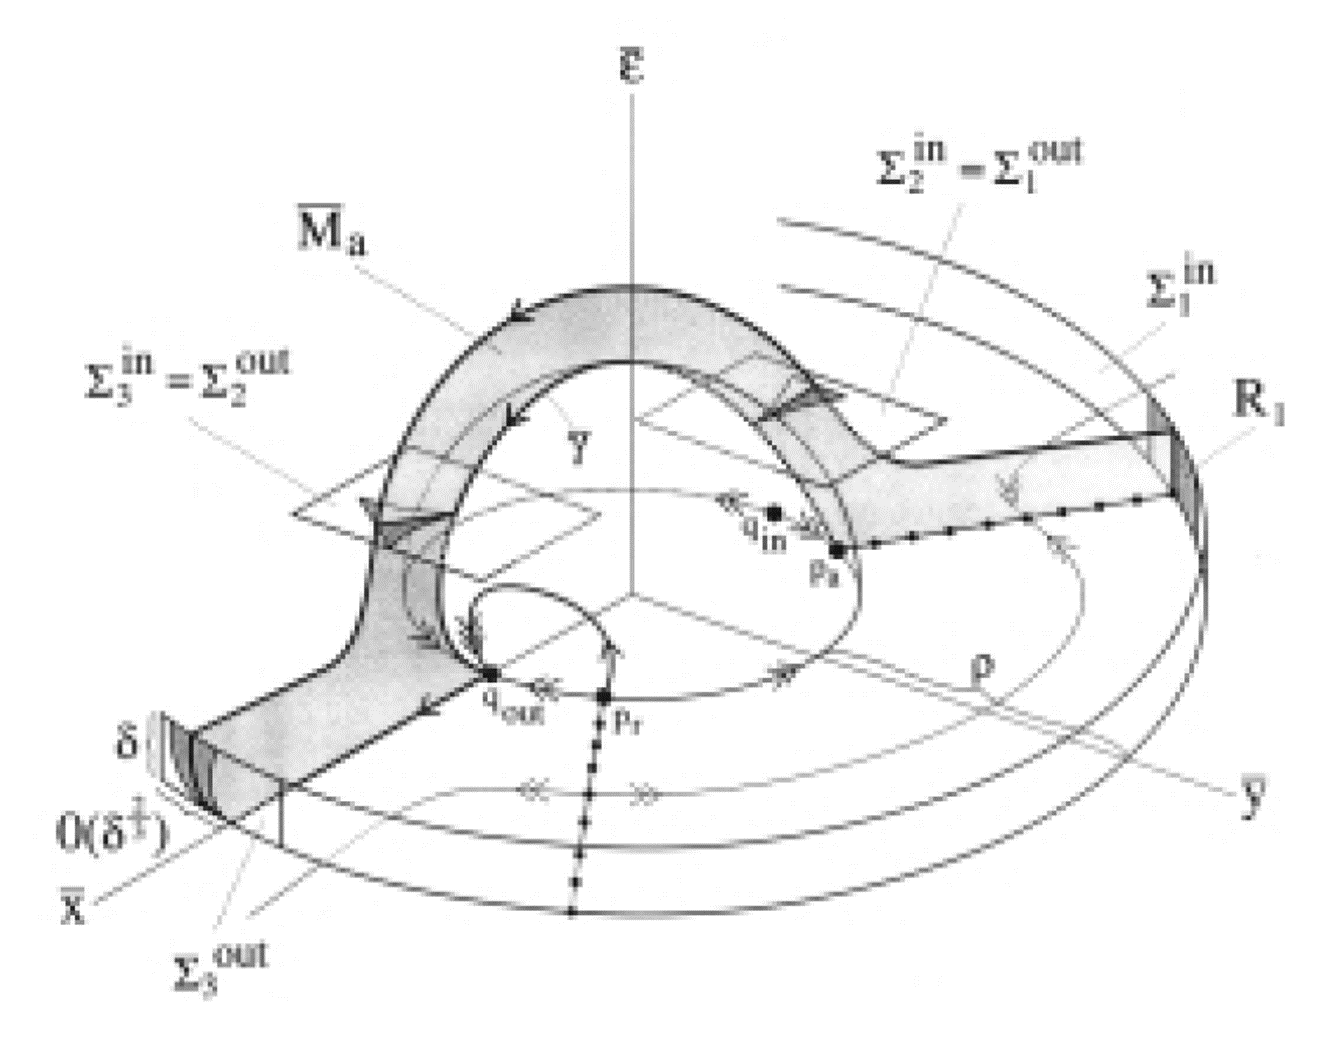
\includegraphics[height=5cm,width=6cm]{Charts.png}
        \caption{Sketch of the coordinate charts (Kuehn, Multiple Time Scale Dynamics)}
    \end{figure}    \column{0.5\textwidth}
        \begin{itemize}
            \item What are charts?
            \item Why use charts?
            \begin{itemize}
                \item Simplifies our singularity
                \item Magnifies our flow 
            \end{itemize}
            \item Transition Maps $\Pi_1\to \Pi_2\to \Pi_1$
        \end{itemize}

    \end{columns}
\end{frame}

\begin{frame}{Dynamics on $K_2$}
\begin{columns}
\column{0.35\textwidth}
\begin{figure}
    \centering
    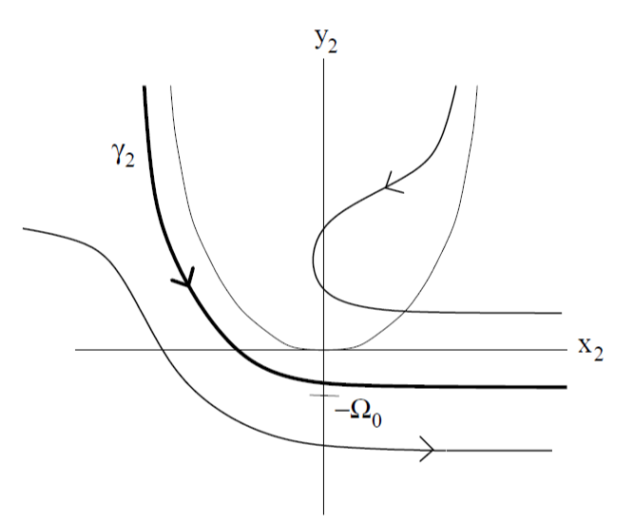
\includegraphics[height=4cm,width=6cm]{Dynamics_in_K2.png}
    \caption{Phase portrait for $\bar{\epsilon}=0$ (Kuehn, Multiple Time Scale Dynamics)}

\end{figure}\column{0.65\textwidth}
\begin{itemize}
\item Transformed Van der Pol equations on $ \epsilon=1$:
\begin{equation*}
    \begin{cases}
        x'_2&=-y_2+x_2^2\\
         y_2'&=x_2-\lambda_2\\
        r'_2&=0\\
        \lambda'_2&=0\\
    \end{cases}
%     G(x_2,y_2)=(G_1(x_1,y_1),G_2(x_2,y_2))^T=(-\frac{x^2_2}{3},0)^T
\end{equation*}
%\item $ x_2' = x_2^2-y_2$
%\item $y_2' = -1$
%\item $r'_2=0$
%\item Matrix of high order terms.
%\begin{itemize}
%\item  $G(x_2,y_2)=(-\frac{x^2_2}{3},0)^T$
%\end{itemize}
\item Constant of Motion in $ K_2 $
\begin{itemize}
	\item $H(x_2,y_2)=\frac{1}{2}e^{(-2y_2)}\left(y_2-x^2_2+\frac{1}{2}\right)$
\end{itemize}
%\begin{itemize}
%\item Mapping trajectories coming from K1 onto trajectories going to K3.
%\item Trajectories follow a Riccati solution on K2.

%\end{itemize}
\end{itemize}
\end{columns}
\end{frame}

\begin{frame}{Dynamics on $K_1$ and the Global Solution}
\begin{columns}
	\column{0.5\textwidth}
	\begin{figure}
		\centering
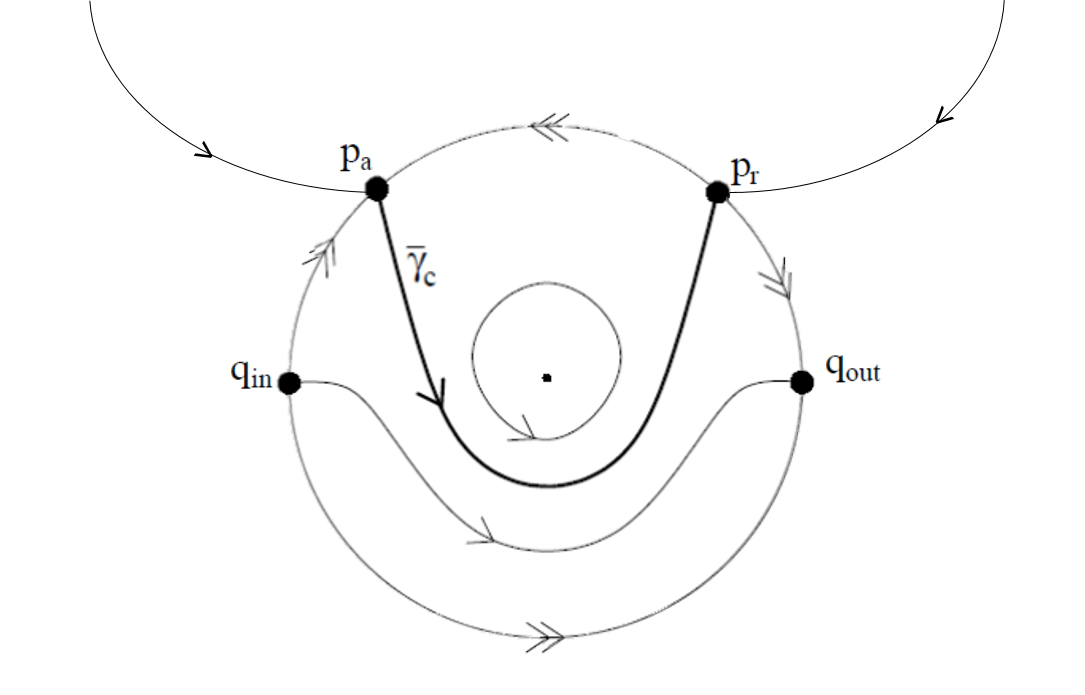
\includegraphics[height=4cm,width=6cm]{Images/pres-cancard}
		\caption{\textbf{Needs changing} (Kuehn, Multiple Time Scale Dynamics)}
		
	\end{figure}\column{0.5\textwidth}
	\begin{itemize}
		\item Transformed Van der Pol equations on $ \epsilon=1$:
		\begin{equation*}
		\begin{cases}
			r_1'&=\frac{\epsilon}{2}(r_1x_1-r_1\lambda_1), \\
		% \label{canard: r1}
		x_1'&=-1+x_1^2-\frac{x_1\epsilon_1F}{2},\\
		\epsilon'&=-\epsilon_1^2F,\\
		\lambda'_1&=-\frac{\lambda_1\epsilon_1F}{2}.
		\end{cases}
		%     G(x_2,y_2)=(G_1(x_1,y_1),G_2(x_2,y_2))^T=(-\frac{x^2_2}{3},0)^T
		\end{equation*}
		%\item $ x_2' = x_2^2-y_2$
		%\item $y_2' = -1$
		%\item $r'_2=0$
		%\item Matrix of high order terms.
		%\begin{itemize}
		%\item  $G(x_2,y_2)=(-\frac{x^2_2}{3},0)^T$
		%\end{itemize}
		\item Trajectories 
		\begin{itemize}
			\item Hopf Bifurcation
			\item Jumps
		\end{itemize}
		%\begin{itemize}
		%\item Mapping trajectories coming from K1 onto trajectories going to K3.
		%\item Trajectories follow a Riccati solution on K2.
		
		%\end{itemize}
	\end{itemize}
\end{columns}
\end{frame}




% \begin{frame}{Dynamics of $K_1$}
% \begin{columns}
% \column{0.4\textwidth}
% \begin{figure}
%     \centering
%     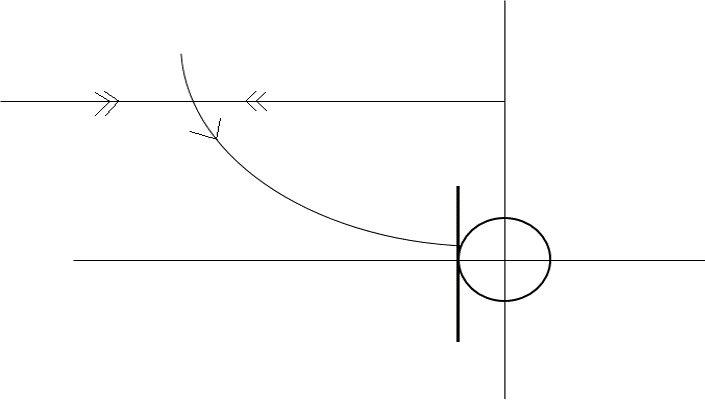
\includegraphics[height=4cm,width=5cm]{Chart_K_1_arrows_Chart.png}
%     \caption{The attracting branch connecting to the blow up.}

% \end{figure}
% \column{0.6\textwidth}
% \begin{itemize}
% \item Connecting the Riccati Flow with the global dynamics on S$^a$.
% \item Transformed Van der Pol Equations:
% \begin{equation}
% 	\begin{cases}
% 		 &x_1' = -1 +x_1^2 + \frac{1}{2} x_1 \epsilon_1 + O(r_1)\\
% 		 &r_1'= \frac{1}{2} r_1 \epsilon_1(-1 +O(r_1) \\
% 		 &\epsilon_1' = \frac{2}{3}\epsilon_1^2(1- O(r_1))
% 	 \end{cases}
% \end{equation}
% \item Cannot solve explicitly.
% \end{itemize}
% \end{columns}
% \end{frame}

% \begin{frame}{Dynamics of $K_1$}
% \begin{columns}
% \column{0.5\textwidth}
% Chart Picture
% \column{0.5\textwidth}
% \begin{itemize}
% \item Invariant Van der Pol:
% \begin{itemize}
% \item $r_1'=0 \ \text{and} \ \epsilon_1'=0$
% \begin{equation}
% \begin{aligned}
%  &x_1' = -1 +x_1^2 + \frac{1}{2} x_1 \epsilon_1 + O(r_1)\\
%  &r_1'= 0 \\
%  &\epsilon_1' = 0
%  \end{aligned}
% \end{equation}
% %item $x_1' = -1 +x_1^2 + \frac{1}{2} x_1 \epsilon_1 + O(r_1)$
% %\item $r_1'= 0 $
% %\item $\epsilon_1' = 0$
% \end{itemize}
% %\item Analysing invariant planes: $r'_1 =0$ and $\epsilon'_1=0$.
% \item Center Manifold Theorem
% \begin{itemize}
% \item Finding equilibria, eigenvalues and eigenvectors.
% \end{itemize}
% \item Deduce existence of $\Pi_1$, connecting S$^a$ and $K_2$.

% \end{itemize}
% \end{columns}
% \end{frame}

% \begin{frame}{Flow on the Charts: K3}
% \begin{columns}
% \column{0.5\textwidth}
% Chart Picture
% \column{0.5\textwidth}
% Dynamics on Chart 3
% \begin{itemize}
% \item Connecting Riccati solution in K2 with global dynamics on S$^r$.
% \item Transformed Van der Pol Equations:
% \begin{itemize}
% \item 
% \item
% \item
% \end{itemize}
% \item Not solvable explicitly.
% \end{itemize}
% \end{columns}
% \end{frame}


% \begin{frame}{Flow on the Charts: K3}
% \begin{columns}
% \column{0.5\textwidth}
% Chart Picture
% \column{0.5\textwidth}
% Dynamics on Chart 3
% \begin{itemize}

% \item Transformed Van der Pol Equations:
% \begin{itemize}
% \item 
% \item
% \item
% \end{itemize}
% \item A map $\Pi_3$ exists.
% \item Can be calculated explicitly. (???)
% \item Maps Riccati trajectories from K2 onto flow around S$^r$.
% \end{itemize}
% \end{columns}
% \end{frame}

\begin{frame}{Effects of a Canard}
\begin{columns}
\column{0.5\textwidth}
\begin{figure}
    
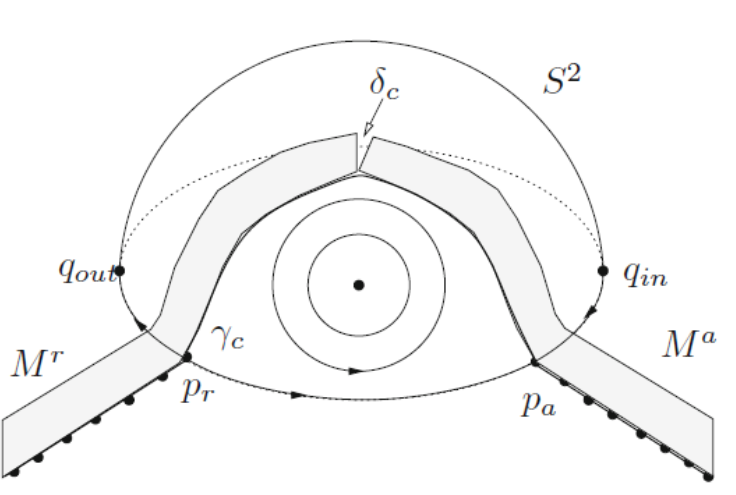
\includegraphics[height=5cm,width=7cm]{Images/Separation}
    \caption{Separation of $ M_a $ and $ M_r $ \citep{Kuehn}.}

\end{figure}\column{0.5\textwidth}
\begin{itemize}
%\item The maps $\Pi_1, \Pi_2, \Pi_3$ can be combined into a global map $\Pi$ using the variable transformations.
\item $\Pi$ describes the global transition of trajectories.
\begin{itemize}
    \item $\Pi=\Pi_3\circ\kappa_{23}\circ\Pi_2\circ\kappa_{12}\circ\Pi_1$
\end{itemize}
% \item Riccati flow at $\bar{\gamma}.$
\item What does $q_{out}$ do?
% \item This describes the flow at $(x^*,y^*)=(0,0)$. %(not on but around???)
\end{itemize}
\end{columns}
\end{frame}

\begin{frame}{Canard Points and Future Work}
\begin{onlyenv}<1>
\begin{equation*} 
        \begin{cases}
        \epsilon\frac{\dif x}{\dif \tau} &= -y + x^2 - \frac{x^3}{3}\\ 
        \frac{\dif y}{\dif \tau}&= (-1+x)
        \end{cases}
        \end{equation*}
\end{onlyenv}

\begin{onlyenv}<2>
    \begin{equation*}
         \begin{cases}
        \epsilon\frac{\dif x}{\dif \tau} &= -y + x^2 - \frac{x^3}{3}\\ 
        \frac{\dif y}{\dif \tau}&= (-\lambda+x)
        \end{cases}
        \end{equation*}
\end{onlyenv}

\begin{onlyenv}<3>
\begin{columns}
\column{0.5\textwidth}
\begin{figure}
    \centering
\includemedia[width=1\linewidth,height=1\linewidth,activate=pageopen,
passcontext,
transparent,
addresource=vdPhopf.mp4,
flashvars={source=vdPhopf.mp4}
]{}{VPlayer.swf}

\end{figure}
\column{0.5\textwidth}
\begin{figure}
    \centering
\includemedia[width=1\linewidth,height=1\linewidth,activate=pageopen,
passcontext,
transparent,
addresource=vdPe001.mp4,
flashvars={source=vdPe001.mp4}
]{}{VPlayer.swf}
    %\caption{Phase Plane of the Van der Pol Equations}
\end{figure}
 

\end{columns}
\begin{equation*} 
        \begin{cases}
        \epsilon\frac{\dif x}{\dif \tau} &= -y + x^2 - \frac{x^3}{3}\\ 
        \frac{\dif y}{\dif \tau}&= (-\lambda+x)
        \end{cases}
        \end{equation*}
\end{onlyenv}
\end{frame}

\begin{frame}{Conclusion}
\begin{itemize}
    \item Lotka-Volterra 
    \item Van der Pol 
    \item Blow ups 
    \item Canard Point
\end{itemize}
\end{frame}

\bibliographystyle{agsm}
\end{document}